\documentclass[12pt,letterpaper]{article}

\usepackage[authoryear]{natbib}
\usepackage{times}
\usepackage{amsmath,amsfonts}
\usepackage{graphicx}
\usepackage{setspace}
\usepackage{indentfirst}
\usepackage{url}
\usepackage{epstopdf}
\usepackage{lineno}
\usepackage{subfig}
\usepackage{comment}

\usepackage[top=1in, bottom=1in, left=1in, right=1in]{geometry}
\setlength{\rightskip}{0pt plus 1fil} % makes ragged right
\doublespacing
\linenumbers
\usepackage{titlesec}
\titleformat*{\section}{\bfseries\sffamily}
\titleformat*{\subsection}{\bfseries\sffamily}

% bibliography format
\usepackage[authoryear]{natbib}
\bibpunct{(}{)}{;}{a}{}{,}

\newcommand{\LOD}{\text{LOD}}
\newcommand{\pLOD}{\text{pLOD}}

% hanging environment for Figure legends
\newenvironment{hanging}
{\begin{list}{}
        {\setlength{\labelwidth}{0in}
         \setlength{\leftmargin}{1em}
         \setlength{\itemindent}{-1em}
        }
}
{\end{list}}

\title{Treatment of the X chromosome in \\
mapping multiple quantitative trait loci}

\author{Quoc Tran$^{*}$, Karl W. Broman$^{\dagger,1}$}

\date{$^*$Department of Statistics, and $^\dagger$Department of
Biostatistics and Medical Informatics,
University of Wisconsin--Madison, Madison, Wisconsin
53706}



\begin{document}
\maketitle


\noindent \textbf{$^{1}$Corresponding Author:} Karl W Broman, Department of
Biostatistics and Medical Informatics, University of
Wisconsin--Madison, 2126 Genetics-Biotechnology Center, 425 Henry
Mall, Madison, WI 53706. E-mail: \verb|broman@wisc.edu|

\bigskip
\noindent \textbf{Running head:} X chromosome in mapping multiple QTL


\bigskip
\noindent \textbf{Key words:} QTL, model selection, X chromosome

\noindent \textbf{ORCID IDs}:
0000-0002-8240-445X (Q.T.);
0000-0002-4914-6671 (K.W.B.)


\clearpage

\section*{ABSTRACT}

Statistical methods to map quantitative trait loci (QTL) often neglect
the X chromosome and may focus exclusively on autosomal loci. But
the X chromosome often requires special treatment: sex and
cross-direction covariates may need to be included to avoid spurious
evidence of linkage, and the X chromosome may require a separate
significance threshold. In multiple-QTL analyses, including the
consideration of epistatic interactions, the X chromosome also
requires special care and consideration. We extend a penalized
likelihood method for multiple-QTL model selection, to appropriately handle the X
chromosome. We examine its performance in simulation and by
application to a large eQTL data set. The method has been implemented
in the package R/qtl.




\clearpage

\section*{INTRODUCTION}

The X chromosome is often neglected in methods to map quantitative
trait loci (QTL), yet it often requires special treatment. For
example, in an intercross between two inbred strains, A and B, the
offspring have genotypes AA, AB, or BB on the autosomes, but on the X
chromosome males are hemizygous A or B, while females have genotypes
either AA or AB, if their paternal grandmother was from strain A, or
genotypes AB or BB, if their paternal grandmother was from strain B.
These differences introduce three difficulties: the treatment of the
male hemizygous genotypes, the potential for spurious evidence for X
chromosome linkage due to a sex or cross-direction difference in the
phenotype, and the need for separate thresholds for statistical
significance for the X chromosome and the autosomes, due to a difference
in degrees of freedom in the linkage tests.
Similar considerations apply in genome-wide association studies
\citep{Zheng2007,Clayton2008,Hickey2011}.

\citet{Broman2006} described the necessary modifications to single-QTL
analysis by interval mapping \citep{Lander1989}. They identified
additional covariates that need to be considered in the null model
with no QTL, to avoid spurious linkage. They identified appropriate
linkage tests for various configurations of an intercross or
backcross, ensuring that the null model is nested within the
alternative, single-QTL model. And they described an approach to
obtain separate permutation-based significance thresholds for the
autosomes and X chromosome.

Many of the difficulties with the X chromosome are further exacerbated
in the consideration of multiple-QTL models. Multiple-QTL models have
a number of advantages for QTL mapping, including the potential for
increased power to detect QTL, the ability to separate linked QTL, and
the possibility of identifying epistatic interactions among QTL. But,
for example, in the consideration of epistatic interactions, the
degrees of freedom for the test for epistasis can vary dramatically
depending on whether both loci are on autosomes, both are on the X
chromosome, or one is on the autosome and one is on the X chromosome
\citep{Broman2009}.

We describe an approach for multiple-QTL model selection, including
the investigation of epistatic interactions, that deals appropriately
with the X chromosome. We build upon the penalized likelihood approach
of \citet{Broman2002} and \citet{Manichaikul2009}. We use permutation
tests \citep{Churchill1994} with two-dimensional, two-QTL genome
scans, to derive separate thresholds for the main effects for QTL on
the autosomes and X chromosome, and for pairwise epistatic
interactions, depending on whether both, one, or neither QTL is on the
X chromosome.

We use computer simulations to assess the performance of our approach.
We further illustrate the approach through application to a large
expression quantitative trait locus (eQTL) study. The method has been
implemented in the widely-used package R/qtl \citep{Broman2003}.




\clearpage
\section*{METHODS}

We consider the case of a backcross or an intercross derived from two
inbred lines and of a continuously varying quantitative trait with
normally distributed residual variation. \citet{Broman2002} introduced
the use of a penalized LOD score criterion for multiple-QTL model
selection in this context. They focused on additive QTL models and
placed a linear penalty on the number of QTL. Their criterion was
$$\pLOD(\gamma) = \LOD(\gamma) - T_m|\gamma|_m$$
where $\gamma$ denotes an additive QTL model, $|\gamma|_m$ is the
number of QTL in the model, and $\LOD(\gamma)$ is the log$_{10}$
likelihood ratio for the model $\gamma$ versus the null model of no
QTL. The penalty $T_m$ was chosen as the $1-\alpha$ quantile of the
genome-wide maximum LOD score in a permutation test
\citep[see][]{Churchill1994}, and they sought the model with maximum
pLOD.

This approach could be modified to allow different penalties for QTL
on the X chromosome than those on autosomes, using significance
thresholds as in \citet{Broman2006}, with $T_{mA}$ and $T_{mX}$ being
the $1-\alpha_A$ and $1-\alpha_X$ quantiles, respectively, of the
maximum LOD scores across the autosomes and the X chromosome, from
a permutation test. \citet{Broman2006} took $\alpha_i = 1
- (1-\alpha_i)^{L_i/L}$, where $L_X$ is the length of the X
chromosome, $L_A$ is the total lengths of the autosomes, and $L = L_A
+ L_X$.


\citet{Manichaikul2009} extended the penalized LOD score approach to
consider models with pairwise interactions among QTL. They imposed a
hierarchy on the models, with the inclusion of a pairwise interaction
requiring the inclusion of both corresponding main effects. We will
also impose this hierarchy. They used the same main-effect penalty as
in \citet{Broman2002}, but added a penalty on interaction terms. They
considered heavy and light penalties on interactions. The heavy
interaction penalty was taken as the $1-\alpha$ quantile of the LOD
score for the interaction term in a two-dimensional, two-QTL scan of
the genome, under the null hypothesis of no QTL. The light interaction
penalty was derived as the $1-\alpha$ quantile for the LOD score
comparing a two-locus interactive model to a single-QTL model, but
then subtracting off the main effect penalty.

The light interaction penalty has the advantage of giving greater
power to detect interactive QTL, but with an increased rate of false
interactions. Exclusive use of the light penalty gave a high rate of
false positive QTL, and so they used a compromise: considering a QTL
model as a graph with nodes being QTL and edges being pairwise
interactions, they allowed no more than one light interaction penalty
for each connected component and placed heavy penalties on all other
interactions.

In adapting the approach of \citet{Manichaikul2009} to handle the X
chromosome, we propose a similar penalized LOD score, but with
separate thresholds for interactions in three regions A:A, A:X,
X:X. \citet{Broman2006} identified sex and cross-direction
covariates that should be included under the null hypothesis; we
include these covariates under all models. The ad hoc system of heavy and
light penalties on interaction terms, suggested by
\citet{Manichaikul2009}, becomes unmanageable when separate
interaction penalties are considered for the three regions, and so we
allow light penalties only for interactions for which both QTL are on
autosomes; any QTL involving the X chromosome must be a heavy penalty.

The main effect penalties are as described above. The interaction
penalties are based on significance levels $\alpha_{AA}$,
$\alpha_{AX}$, $\alpha_{XX}$, based on the areas of the corresponding
regions. For region $i$, we use $\alpha_i = 1 - (1-\alpha)^{S_i/S}$,
where $S_{AA} = L_A^2/2$, $S_{AX} = L_AL_X$, $S_{XX} = L_X^2/2$, and
$S = S_{AA} + S_{AX} + S_{XX}$.

In the following, we denote the method of \citet{Manichaikul2009}
treating the autosomes and X chromosome the same as XeqA (for X
chromosome and autosomes treated equally), and the proposed approach,
treating the X chromosome separately, as XneA.

The proposed approach requires a permutation test with a
two-dimensional, two-QTL genome scan, keeping track of the maximum LOD
score in the three regions, A:A, A:X, and X:X. And as the quantiles
for the A:X and X:X regions are much farther out in the tail, we will
need to perform many more permutations for the A:X and X:X regions in
order to get accurate estimates of the penalties. In
\citet{Broman2006}, they suggested using a factor $L_A/L_X$ additional
permutations for the X chromosome as for autosomes. Following that
approach, we would require $(L_A/L_X)^2$ as many permutations for the
X:X region as for the A:A region.

To search the space of QTL models, we use forward selection up to a
model with 10 QTL, followed by backward elimination to
the null model. At each step of forward selection, we scan the genome
for an additional additive QTL, and then for each QTL in the current
model, we scan the genome for a QTL that interacts with that QTL. We
step to the model that gives the largest penalized LOD score, even if
it results in a decrease relative to the current model. In the end, we
select the model with maximum penalized LOD score, among all models
considered in the search.

\subsection*{Data and software availability}

Software implementing the proposed methods have been incorporated into
the R/qtl package, which is available at its website
(\url{https://rqtl.org}), at GitHub
(\url{https://github.com/kbroman/qtl}), and at the Comprehensive R
Archive Network (CRAN, \url{https://cran.r-project.org}).
The data from \citet{Tian2016}, considered in the Application section
below, are available at
the Mouse Phenome Database, at
\url{https://phenome.jax.org/projects/Attie1}.
The detailed code we used for the simulations and in the application
are available at \url{https://github.com/kbroman/Paper_qtlX}.


\clearpage
\section*{SIMULATIONS}

To investigation the performance of our proposed approach, we
conducted a computer simulation. We compare the Type I error rate and
power, including the relative rates of Type I errors on autosomes
versus the X chromosome.

We consider a backcross with 250 individuals, split evenly between males and females, using a genome modeled
after the mouse, with markers at a 10~cM spacing. We considered a
variety of small QTL models: a single QTL, two additive QTL, or three
additive QTL all on autosomes; a single QTL or two additive QTL on the
X chromosome; two interacting QTL on autosomes; and two interacting
QTL with one on an autosome and one on the X chromosome. In all cases,
the percent phenotypic variance explained by each QTL was
approximately 8\%. We used Haley-Knott regression \citep{Haley1992}
and stepwise model selection. Analyses were performed with R/qtl
version 1.42-8 \citep{Broman2002} and R version 3.5.3 \citep{R}.

%The degree of freedom is in Table~\ref{tab:bcdf}.
First we use simulation to derive the various penalties for the XeqA
and XneA methods. For the XneA methods, we performed 1,056 simulation replicates for the A:A region, 8,544 replicates for the A:X region, and 276,192 replicates for the X:X region. The estimated penalties are shown in Table~\ref{tab:penalties}.
These penalties are used to perform stepwise model selection.
The results, based on 1,000 simulations, are displayed in
Figure~\ref{fig:sim_result}.
Figure~\ref{fig:sim_result}A shows the Type I error rate for main
effect QTL. Treatment of the X chromosome separately from the
autosomes (XneA) results in a smaller Type I error rate than when all
chromosomes are treated equally (XeqA).
The XeqA method has high Type I error rate particularly when  the
simulated model has two main QTL on X chromosome.

Figure~\ref{fig:sim_result}B shows the log$_2$ ratio of Type I error
rates, for the autosomes versus the X chromosome. The proposed XneA
method serves to balance type I error rates on the autosomes and the X
chromosome, while the XeqA method shows increased type I error on the X
chromosome.

Figure~\ref{fig:sim_result}C shows the type I error rate for
interactions. The XneA method is conservative, with below-target rates of
type I errors. The XeqA method has high false type I error rates for interactions,
particularly in the case of two QTL on the X chromosome.

Figure~\ref{fig:sim_result}D shows the power to detect QTL. For
autosomal QTL, the two approaches have similar power. The XneA method
has lower power to detect X chromosome QTL. This is the trade-off to
control the Type I error rate on the X chromosome.



\clearpage
\section*{APPLICATION}

To illustrate our method regarding the X chromosome in multiple-QTL
model selection, we consider the eQTL data of \citet{Tian2016}. The
data concern a mouse intercross between the diabetes-resistance strain
C57BL/6J (abbreviated B6) and the diabetes-susceptible strain
BTBR $T^{+} tf$/J (abbreviated BTBR). There
were approximately 500 F$_2$ offspring, all genetically obese through
introgression of the leptin mutation ($Lep^{ob/ob}$). Genome-wide gene
expression data were available on six tissues, assayed with custom
two-color Agilent microarrays; here, we focus on liver expression, for
which there was data on 483 F$_2$ mice.
Mice were genotyped with the Affymetrix 5K GeneChip, giving 2,057
informative markers.

The F$_1$ parents were derived from a cross between a female BTBR and
a male B6. Thus the female F$_2$ offspring all have an X chromosome
from BTBR and so are either homozygous BTBR or heterozygous. The males
have a Y chromosome from B6 and are hemizygous B6 or BTBR on the X.
%The degree of freedom is in Table~\ref{tab:f2onewaybothsexdf}.

We first used computer simulation to estimate penalties for the XeqA
and XneA methods. For all mice in the study, we simulated standard
normal phenotypes, independent of genotype, and performed
two-dimensional, two-QTL genome scans with sex as an additive
covariate to estimate the various penalties. We performed 1,056
simulation replicates for the A:A region, 9,504 replicates for the A:X
region, and 335,328 replicates for the X:X region. The numbers of
replicates were chosen based on the areas of the corresponding
regions, with $L_A/L_X \approx 19$. Penalties using $\alpha=0.05$ are
displayed in Table~\ref{tab:penalties}.
Note that the number of degrees of freedom for the main-effect QTL test on
the X chromosome, $6$, is less than that on the autosomes, $8$, and so the
main effect penalty on the X chromosome is lower. The interaction
penalty for two QTL on the X chromosome is lower than the heavy
interaction penalty for two QTL on autosomes, but the
penalty for interactions between autosomal and X chromosome QTL is
highest.

We considered the 37,827 gene expression microarray probes with known
genomic location (including 1,433 on the X chromosome, 21 on the Y
chromosome, and 9 mitochondrial probes). The gene
expression values to normal quantiles. We performed single-QTL genome
scans and identified 10,814 microarray probes (29\%) with at least one
significant QTL at $\alpha=0.05$, allowing separate significance
thresholds on the autosomes and X chromosome. For the multiple-QTL
analyses, we will focus on these 10,814 microarray probes.

Table~\ref{tab:num_qtl} shows the distribution of the estimated number
of QTL by the two methods, as well as the estimated number of pairwise
interactions. As we focused on microarray probes with at least one
significant QTL in a single-QTL genome scan allowing separate autosome
and X chromosome thresholds, it is no surprise that all of these
microarray probes showed at least one QTL by the XneA method.

There were 56 microarray probes that showed no QTL by the XeqA method.
All of these showed a single QTL on the X chromosome by the XneA
method. This can be explained by the fact that the main effect penalty
for the X chromosome is considerably smaller than that for the
autosomes (Table~\ref{tab:penalties}).

In general, these expression traits show a large number of QTL. While
about half show a single QTL, about a quarter show 2 QTL and another
quarter show 3 or more QTL. The number of interactions, however, is
quite small. Less than 4\% of expression traits show an interaction,
and about 0.1\% have two or more interactions.

The two methods gave identical results for the vast majority of the
microarray probes: 10,290 (95.2\%) gave the same QTL model by the two
methods, and just 524 (4.8\%) gave different models. For 257
microarray probes (2.4\%), the XneA results were nested within the
XeqA results, while for 98 microarray probes (0.9\%), the XeqA results
were nested within the XneA results. Another 169 (1.6\%) had more
complex differences, with some gains and losses on both sides.
In 139 of the 524 cases where the two methods gave different results,
part of the difference included the X chromosome: 86 microarray probes
gained an X chromosome QTL by the XneA method, while 53 lost an X
chromosome QTL.

As one example of the kinds of differences observed, consider
microarray probe 10003837305, which is on chromosome 1 at 152~Mb
(63.2~cM), though not in a known gene. The results by the two methods
are in Table~\ref{tab:p10003837305}, with the results by the XeqA
method on the left, and those for the XneA method on the right.
By the XeqA method, there are two QTL on chromosome 7, one of which
interacts with a locus on the X chromosome. With the XneA method, the
QTL on chromosome 7 with the 7:X interaction is omitted, and instead
there is an interaction between the other chromosome 7 QTL and the
locus on chromosome 10. The position of the chromosome 10 QTL shifts a
bit, but the positions of most other QTL do not change much. Note that
the QTL on chromosome 1 is very close to the genomic location for this
microarray probe.

Figure~\ref{fig:probe305} shows LOD profiles for the two models for
this microarray probe, with results for the XneA method in green. Each
curve shows the log$_{10}$ likelihood when varying the position of the
given QTL, keeping all other QTL fixed at their estimated positions,
versus the model where the given QTL is omitted (along with any
interactions it is involved in). These curves show the strength of
evidence for the QTL as well as an indication of their mapping
precision. Again, in switching from the XeqA method to the XneA
method, one of the chromosome 7 QTL is lost, as is the 7:X
interaction, but a 7:10 interaction is gained, and the position of the
chromosome 10 QTL shifts.


\clearpage
\section*{DISCUSSION}

We have introduced an approach for multiple-QTL model selection that
takes account of the X chromosome. It builds on the penalized LOD
score method of \citet{Manichaikul2009}, but with a separate
main-effect penalty for the autosomes and the X chromosome, and
separate interaction penalties for the three kinds of pairwise
interactions: between two autosomal QTL, between two X chromosome QTL,
and between a QTL on an autosome and one on the X chromosome.

Our approach balances false positive rates between the autosomes and
the X chromosome. In our computer simulations, which concerned a
backcross with both sexes, the main effect penalty is higher for the X
chromosome than for autosomes, and so the new approach gives a loss of
power to detect QTL on the X chromosome. The application to the
eQTL dataset of \citet{Tian2016} concerned an intercross with both
sexes but just one cross direction, and so the main effect penalty was
lower for the X chromosome than for autosomes, and so the new approach
gave some additional QTL on the X chromosome.

In the eQTL application, for the vast majority of expression traits,
the separate treatment of the X chromosome gave identical results.
This is as expected: the penalties (Table~\ref{tab:penalties}) have
relatively small changes, and these changes will only affect the
results when loci or interactions have LOD scores in-between these
penalty values.

In the eQTL application, many expression traits showed multiple QTL,
including up to 10 QTL. (Our model search did not consider models with
more than 10 QTL.) However, there were few expression traits for which
we identified epistatic interactions. The high degrees of freedom of
the test for epistatic interactions in an intercross, as well as large
search space, result in large penalties on interactions and so low
power to detect interactions.

Software implementing our approach has been incorporated into
R/qtl \citep{Broman2003}, an add-on package
to the general statistical software R \citep{R}.

\section*{ACKNOWLEDGMENTS}

This work was supported in part by National Institutes of Health
grants R01GM074244 and R01GM070683 (to K.W.B.).


\clearpage
\bibliographystyle{genetics}
\renewcommand*{\refname}{LITERATURE CITED}
\bibliography{qtlX}



%%%%%%%%%%%%%%%%%%%%%%%%%%%%%%%%%%%%%%%%%%%%%%%%%%%%%%%%%%%%%%%%%%%%%%
% TABLES
%%%%%%%%%%%%%%%%%%%%%%%%%%%%%%%%%%%%%%%%%%%%%%%%%%%%%%%%%%%%%%%%%%%%%%
\clearpage
\begin{comment}
\begin{table}
\begin{center}
  \caption{Degree of freedom for backcross.\label{tab:bcdf}}

    \begin{tabular}{cccccc}
    \cline{1-6}
    \textbf{Area} & \textbf{f} & \textbf{fv1} & \textbf{i} & \textbf{a} & \textbf{av1} \\
    A:A &   3 &    2 & 1 & 2 & 1 \\
    A:X &   6 &    4 & 2 & 4 & 2 \\
    X:X &   6 &    4 & 2 & 4 & 2 \\
    \cline{1-6}
  \end{tabular}
\end{center}
\end{table}

\begin{table}
\begin{center}
  \caption{Degree of freedom for intercross with one directions and both sexes.\label{tab:f2onewaybothsexdf}}

    \begin{tabular}{cccccc}
    \cline{1-6}
    \textbf{Area} & \textbf{f} & \textbf{fv1} & \textbf{i} & \textbf{a} & \textbf{av1} \\
    A:A &   8 &    6 & 4 & 4 & 2 \\
    A:X &   10&    8& 4& 6 & 4 \\
    X:X &   6 &    4 & 2 & 4 & 2 \\
    \cline{1-6}
  \end{tabular}
\end{center}
\end{table}
\end{comment}

\begin{table}
\begin{center}
  \caption{Estimated penalties for the simulations and the
    application, for the XeqA and XneA methods.\label{tab:penalties}}

  \begin{tabular}{cccccc} \hline
             & \multicolumn{2}{c}{\textbf{Simulations}} &\quad&
    \multicolumn{2}{c}{\textbf{Application}} \\ \cline{2-3} \cline{5-6}
    \textbf{Penalty} & \textbf{XeqA} & \textbf{XneA} && \textbf{XeqA}
    & \textbf{XneA} \\ \hline
    T$_{mA}$    & 2.98 & 2.88 && 3.85 & 3.90 \\
    T$_{mX}$    &      & 3.61 &&      & 3.51 \\
    T$_{iAA}^H$ & 4.83 & 4.34 && 6.69 & 6.59 \\
    T$_{iAA}^L$ & 2.28 & 1.83 && 3.73 & 3.62 \\
    T$_{iAX}$   &      & 5.74 &&      & 7.21 \\
    T$_{iXX}$   &      & 5.15 &&      & 4.88 \\ \hline
  \end{tabular}
\end{center}
\end{table}



\clearpage

\begin{table}
\begin{center}
  \caption{Distribution of the estimated number of QTL and pairwise interactions for the
    liver expression data from \citet{Tian2016}, for the 10,814 gene
    expression microarray probes with at least one QTL by the XneA
    method.\label{tab:num_qtl}}

  \begin{tabular}{crrccrr}
    \cline{1-3}\cline{5-7}
    \textbf{No. QTL} & \textbf{XeqA} & \textbf{XneA} & \qquad\qquad &
    \textbf{No. interactions} & \textbf{XeqA} & \textbf{XneA} \\
    \cline{1-3}\cline{5-7}
    0 &   56 &    0 && 0 & 10408 & 10419 \\
    1 & 5212 & 5432 && 1 &   392 &   380 \\
    2 & 2566 & 2518 && 2 &    12 &    13 \\
    3 & 1444 & 1397 && 3 &     2 &     2 \\ \cline{5-7}
    4 &  732 &  712 &\\
    5 &  390 &  373 &\\
    6 &  205 &  194 &\\
    7 &  114 &  116 &\\
    8 &   46 &   45 &\\
    9 &   26 &   25 &\\
   10 &   23 &    2 &\\ \cline{1-3}
  \end{tabular}
\end{center}
  \end{table}






\clearpage
\begin{table}
\caption{Comparison of the selected QTL models by the XeqA and XneA methods,
  on probe 10003837305.\label{tab:p10003837305}}

\subfloat[XeqA]{\centering
\begin{tabular}[t]{l|l|l|r|r}
\hline
  & name & chr & pos & LOD\\
\hline
Q1 & 1@60.0 & 1 & 60.0 & 5.4\\
\hline
Q2 & 7@2.5 & 7 & 2.5 & 10.7\\
\hline
Q3 & 7@20.1 & 7 & 20.1 & 5.8\\
\hline
Q4 & 9@31.6 & 9 & 31.6 & 7.1\\
\hline
Q5 & 10@3.0 & 10 & 3.0 & 4.0\\
\hline
Q6 & 13@14.4 & 13 & 14.4 & 5.4\\
\hline
Q7 & 17@19.6 & 17 & 19.6 & 7.1\\
\hline
Q8 & X@57.4 & X & 57.4 & 42.1\\
\hline
Q2:Q8 & 7@2.5:X@57.4 & 7:X &  & 6.4\\
\hline
\end{tabular}
} \quad
\subfloat[XneA]{ \centering
\begin{tabular}[t]{l|l|l|r|r}
\hline
  & name & chr & pos & LOD\\
\hline
Q1 & 1@59.3 & 1 & 59.3 & 5.0\\
\hline
Q2 & 7@18.6 & 7 & 18.6 & 15.1\\
\hline
Q3 & 9@31.6 & 9 & 31.6 & 5.6\\
\hline
Q4 & 10@24.0 & 10 & 24.0 & 8.7\\
\hline
Q5 & 13@14.4 & 13 & 14.4 & 4.4\\
\hline
Q6 & 17@13.1 & 17 & 13.1 & 5.7\\
\hline
Q7 & X@56.4 & X & 56.4 & 34.5\\
\hline
Q2:Q4 & 7@18.6:10@24.0 & 7:10 &  & 7.0\\
\hline
\end{tabular}
}

\end{table}



%%%%%%%%%%%%%%%%%%%%%%%%%%%%%%%%%%%%%%%%%%%%%%%%%%%%%%%%%%%%%%%%%%%%%%
% FIGURES
%%%%%%%%%%%%%%%%%%%%%%%%%%%%%%%%%%%%%%%%%%%%%%%%%%%%%%%%%%%%%%%%%%%%%%
\clearpage
\begin{figure}
\centering
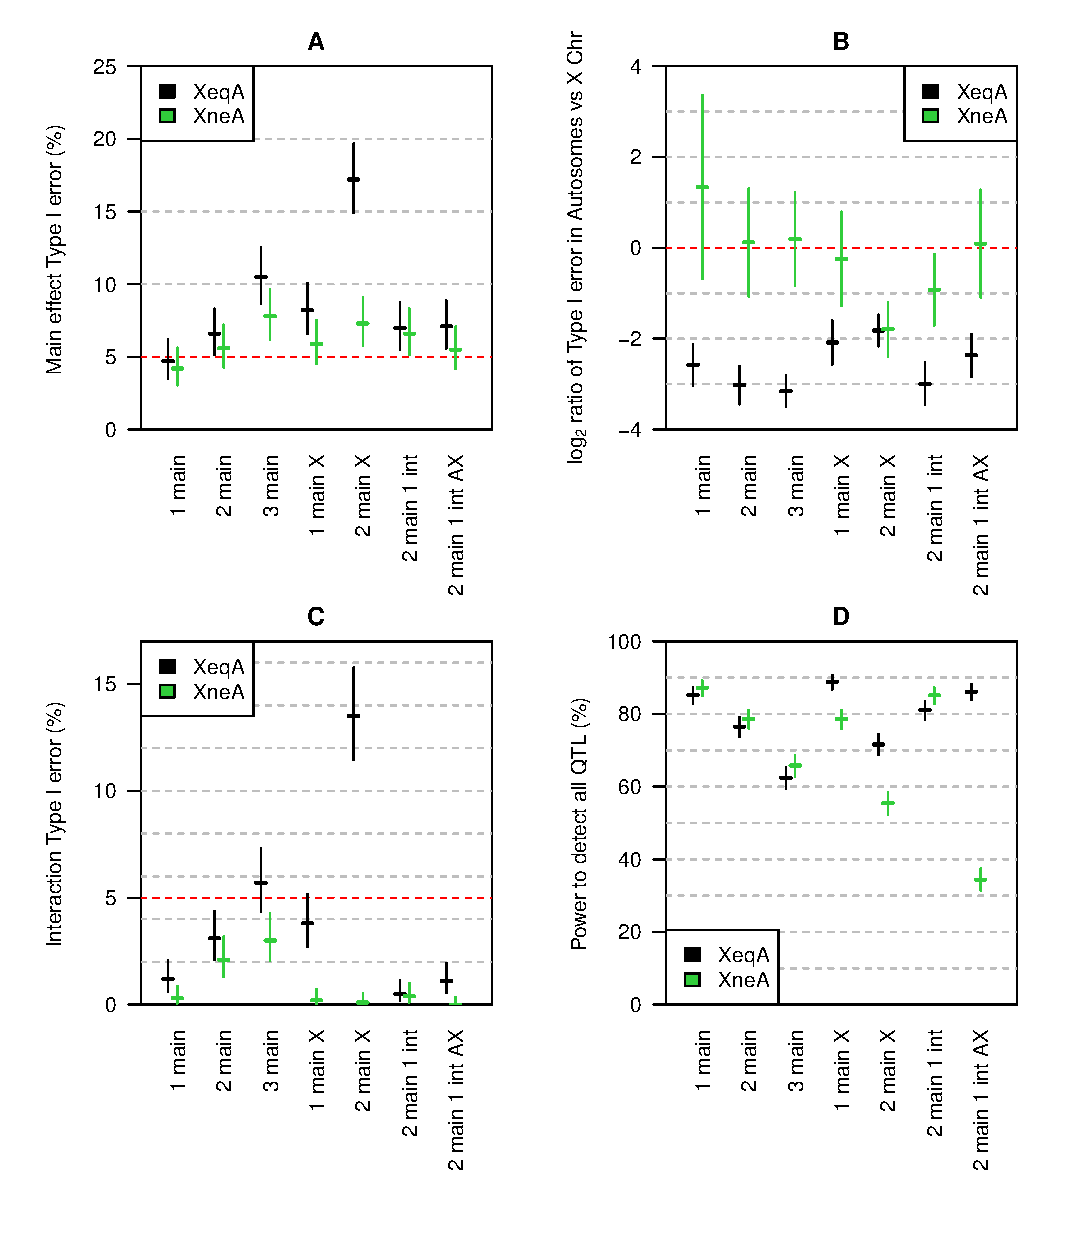
\includegraphics[width=\textwidth]{Figs/fig_sim.eps}

\vspace{0cm}

\caption{Simulation results: Type I error and power of these methods
  across simulated models. Black is the method treating the X
  chromosome and autosomes the same (XeqA); green is the method
  treating the X chromosome and autosomes differently (XneA).
  The estimates and 95\% confidence intervals are based on 1000 simulations.
  A: Type I error for main effects. B: log$_2$ ratio of the
  Type I error of main effects for autosomes versus the X
  chromosome. C: Type I error for interactions.
  D: Power to detect QTL.
\label{fig:sim_result}}
\end{figure}



\clearpage
\begin{figure}
\centering
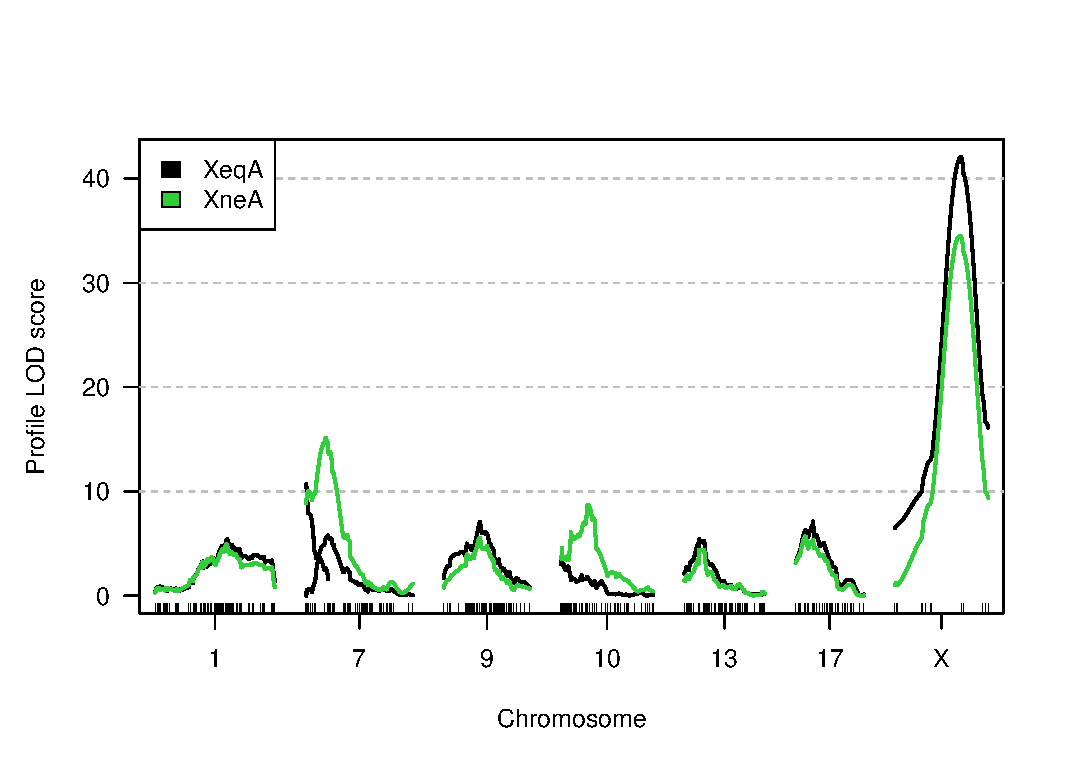
\includegraphics[width=\textwidth]{Figs/fig_prob305.eps}

\vspace{0cm}

\caption{LOD profile of output models from XeqA and XneA methods
  on probe 10003837305.
\label{fig:probe305}}
\end{figure}



\end{document}
